\documentclass[11pt]{beamer}
\usepackage{amsmath, amsfonts, amscd, amssymb, amsthm, tikz,pgfplots}
\usepackage{array}

\usetheme{eaperry}
%\usetheme{CoeCollege}

%\bibliographystyle{aer}
\usepackage{natbib}

\title{A Theory of Investment for\\ Energy-Efficient Technologies}
\subtitle{Part III}
\author{Evan Perry}
\institute{Spellman Program}
\date{June 29, 2021}

\begin{document}

\maketitlepage

\begin{frame}{Review}

\begin{exampleblock}{\large\textbf{Research Question}}
How do neighborhood characteristics relate to the number of certified energy-efficient commercial buildings?
\end{exampleblock}

\vfill
Last Week:
\begin{itemize}
	\item The Energy-Efficiency Gap
	\item Future Energy Savings v. Upfront Costs
	\item Still Focusing on Energy-Using Durables
\end{itemize}
\end{frame}

\begin{frame}{Paper}

{\bf Eichholtz, Piet, Nils Kok, and John~M Quigley}, ``Doing well by\\
\quad doing good? Green office buildings,'' {\it American Economic\\ \quad Review}, 2010, {\it
  100} (5), 2492--2509.

\vfill
\begin{itemize}
	\item Similar ideas, but much closer to my research question
	\item An extra incentive problem with buildings
\end{itemize}

\end{frame}


\begin{frame}{Overview}

\begin{description}
	\item[Purpose] Will firms pay more for green buildings? For what reasons?
	\vfill
	
	\item[Model] Use a standard hedonic pricing model for office building rents 
	\vfill
	
	\item[Method] Identify green buildings and nearby non-green buildings, and estimate the model to find the predicted difference in rents
	\vfill
	
	\item[Results] 3\% premium on the rent per sq. ft.
\end{description}

\end{frame}

\newsection{Background}{\textit{Adoption}}

\begin{frame}{The Scope of Commercial Green Buildings}

\begin{figure}
\centering
\caption{Certified Green Office Space -- 30 Largest Markets \citep{GBAI2019}}
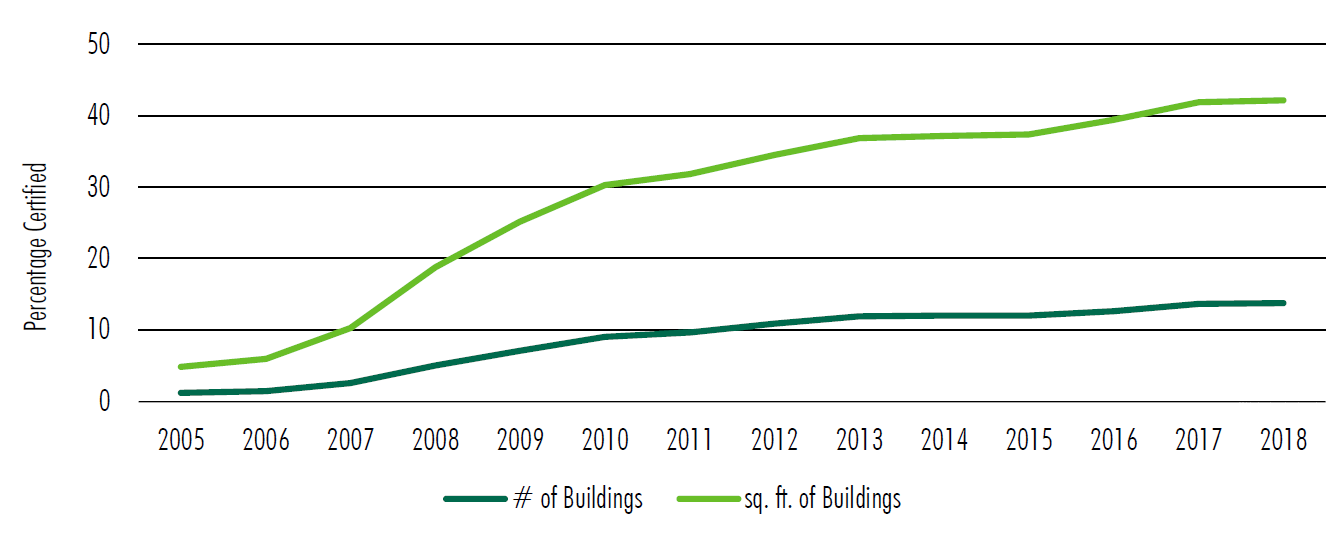
\includegraphics[width = \linewidth]{certOfficeSpace.png}
\end{figure}

\end{frame}


%\begin{frame}{Explaining the Rise in Green Building}
%
%\begin{enumerate}
%	\item For the Occupant,  Less Spending on Energy
%	\vfill
%	\item For the Owner, Protect Against Future Regulation
%	\vfill	
%	\item For Both, Build a Reputation as ``Green"
%	\begin{itemize}
%		\item Attract employees and investors
%		\item e.g. \href{https://sustainability.google/commitments/}{Google}
%	\end{itemize}
%\end{enumerate}
%
%\end{frame}


\newsection{Method}{\textit{Data and Econometric Model}}


\begin{frame}{Data}
\begin{columns}
\begin{column}{0.6\linewidth}
\begin{itemize}
	\item Energy Star Program \& LEED (Leadership in Energy and Environmental Design)
	\begin{itemize}
		\item Two Largest Green Building Rating Programs
		\item 694 Buildings
	\end{itemize}
	\vspace{1.5cm}
	\item CoStar
	\begin{itemize}
		\item Commercial Real Estate Service
		\item 7,411 Nearby Buildings
	\end{itemize}
\end{itemize}
\end{column}
\begin{column}{0.4\linewidth}
\centering
\begin{figure}
\caption{Example Cluster in Chicago}
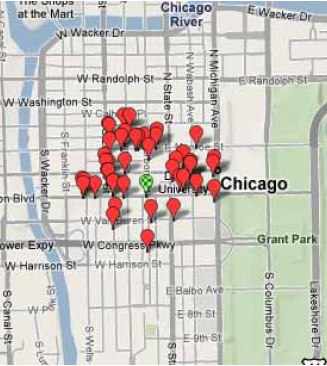
\includegraphics[width=\textwidth]{she-cago.png}
\scriptsize \citep{eichholtz2011rents}
\end{figure}
\end{column}
\end{columns}
\end{frame}


\begin{frame}{Econometric Model}

\[
\log R_{in} = \alpha + \beta_i \textbf{X}_i + \sum_{n=1}^{N} \gamma_n c_n + \textcolor{EAPblue}{\pmb \delta} g_i + \varepsilon_{in}
\]

\small
\begin{itemize}
	\item $i$ : Office Building
	\item $n$ : Office Building Cluster
	\item $R$ : Rent / Sq. ft. of Building $i$ in Cluster $n$
	\item  $\textbf{X}_i$ : Column Vector of Building Characteristics for $i$
	\item $c_n$ : Dummy Variable for Cluster $n$
	\item  $g_i$ : Green Dummy Variable
\end{itemize}

\end{frame}


\newsection{Results}{}


%\begin{frame}{}
%\begin{table}
%\caption{Regression Results \citep{eichholtz2010doing}}
%\scriptsize
%\begin{tabular}{p{0.3\linewidth} >{\centering\arraybackslash}p{0.12\textwidth} >{\centering\arraybackslash}p{0.12\textwidth} >{\centering\arraybackslash}p{0.12\textwidth} >{\centering\arraybackslash}p{0.12\textwidth}}
%\multicolumn{5}{c}{\textit{Dependent Variable: Log Rent /sq.ft.}}\\
%\hline\hline
% & (1) & (2) & (3) & (4) \\
%\hline
%	Green rating & 0.035 &  & \\
%	(Yes = 1) & (0.009) & & \\ \\[-1.2ex]
%	\qquad \textcolor{black!20!}{Energy Star} & &  \\
%	\qquad \textcolor{black!20!}{(Yes = 1)} & &  \\ \\[-1.2ex]
%	\qquad \textcolor{black!20!}{LEED} & & \\
%	\qquad \textcolor{black!20!}{(Yes = 1)} & &  \\ \\[-1.2ex]
%	Building Size & 0.113 & \\
%	(millions of sq.ft.)& (0.019) &  \\ \\[-1.2ex]
%	\textcolor{black!20!}{Age $< 10$ years} &  &   \\
%	\textcolor{black!20!}{(Yes = 1)} & & & \\\\[-1.2ex]
%	\textcolor{black!20!}{Amenities} & & & & \\
%	\textcolor{black!20!}{(Yes = 1)} & & & & \\\\[-1.2ex]
%	Sample Size & 8,105 &  \\
%	R$^2$ & 0.72  \\
%	Adj. R$^2$ & 0.69 \\
%	\hline \hline
%\end{tabular}
%\end{table}
%\scriptsize{Standard errors in parentheses}
%\end{frame}
%
%\addtocounter{framenumber}{-1}
%\setcounter{table}{0}
%
%\begin{frame}{}
%\begin{table}
%\caption{Regression Results \citep{eichholtz2010doing}}
%\scriptsize
%\begin{tabular}{p{0.3\linewidth} >{\centering\arraybackslash}p{0.12\textwidth} >{\centering\arraybackslash}p{0.12\textwidth} >{\centering\arraybackslash}p{0.12\textwidth} >{\centering\arraybackslash}p{0.12\textwidth}}
%\multicolumn{5}{c}{\textit{Dependent Variable: Log Rent /sq.ft.}}\\
%\hline\hline
% & (1) & (2) & (3) & (4) \\
%\hline
%	Green rating & 0.035 &  & \\
%	(Yes = 1) & (0.009) & & \\ \\[-1.2ex]
%	\qquad Energy Star & & 0.033 & & \\
%	\qquad (Yes = 1)& & (0.009) & & \\ \\[-1.2ex]
%	\qquad LEED & & 0.052 & & \\
%	\qquad (Yes = 1) & & (0.036) & & \\ \\[-1.2ex]
%	Building Size & 0.113 & 0.113 & \\
%	(millions of sq.ft.)& (0.019) & (0.019)  &  \\ \\[-1.2ex]
%	\textcolor{black!20!}{Age $< 10$ years} &  &  & \\
%	\textcolor{black!20!}{(Yes = 1)} & & & \\\\[-1.2ex]
%	\textcolor{black!20!}{Amenities} & & & & \\
%	\textcolor{black!20!}{(Yes = 1)} & & & & \\\\[-1.2ex]
%	Sample Size & 8,105 & 8,105 &  \\
%	R$^2$ & 0.72 & 0.72  & \\
%	Adj. R$^2$ & 0.69 & 0.69 &  \\
%	\hline \hline
%\end{tabular}
%\end{table}
%\scriptsize{Standard errors in parentheses}
%\end{frame}
%
%\addtocounter{framenumber}{-1}
%\setcounter{table}{0}
%
%\begin{frame}{}
%\begin{table}
%\caption{Regression Results \citep{eichholtz2010doing}}
%\scriptsize
%\begin{tabular}{p{0.3\linewidth} >{\centering\arraybackslash}p{0.12\textwidth} >{\centering\arraybackslash}p{0.12\textwidth} >{\centering\arraybackslash}p{0.12\textwidth} >{\centering\arraybackslash}p{0.12\textwidth}}
%\multicolumn{5}{c}{\textit{Dependent Variable: Log Rent /sq.ft.}}\\
%\hline\hline
% & (1) & (2) & (3) & (4) \\
%\hline
%	Green rating & 0.035 &  & 0.033 & \\
%	(Yes = 1) & (0.009) & & (0.009) & \\ \\[-1.2ex]
%	\qquad Energy Star & & 0.033 & & \\
%	\qquad (Yes = 1)& & (0.009) & & \\ \\[-1.2ex]
%	\qquad LEED & & 0.052 & & \\
%	\qquad (Yes = 1) & & (0.036) & & \\ \\[-1.2ex]
%	Building Size & 0.113 & 0.113 & 0.102 &\\
%	(millions of sq.ft.)& (0.019) & (0.019)  & (0.019)  & \\ \\[-1.2ex]
%	Age $< 10$ years &  &  & 0.118 &  \\
%	(Yes = 1) & & & (0.016) & \\\\[-1.2ex]
%	\textcolor{black!20!}{Amenities} & & & & \\
%	\textcolor{black!20!}{(Yes = 1)} & & & & \\\\[-1.2ex]
%	Sample Size & 8,105 & 8,105 &  8,105\\
%	R$^2$ & 0.72 & 0.72  & 0.72 & \\
%	Adj. R$^2$ & 0.69 & 0.69 & 0.69  \\
%	\hline \hline
%\end{tabular}
%\end{table}
%\scriptsize{Standard errors in parentheses}
%\end{frame}
%
%\addtocounter{framenumber}{-1}
%\setcounter{table}{0}

\begin{frame}{}
\begin{table}
\caption{Regression Results \citep{eichholtz2010doing}}
\scriptsize
\begin{tabular}{p{0.3\linewidth} >{\centering\arraybackslash}p{0.12\textwidth} >{\centering\arraybackslash}p{0.12\textwidth} >{\centering\arraybackslash}p{0.12\textwidth} >{\centering\arraybackslash}p{0.12\textwidth}}
\multicolumn{5}{c}{\textit{Dependent Variable: Log Rent /sq.ft.}}\\
\hline\hline
 & (1) & (2) & (3) & (4) \\
\hline
	Green rating & 0.035 &  & 0.033 & 0.028\\
	(Yes = 1) & (0.009) & & (0.009) & (0.009)\\ \\[-1.2ex]
	\qquad Energy Star & & 0.033 & & \\
	\qquad (Yes = 1)& & (0.009) & & \\ \\[-1.2ex]
	\qquad LEED & & 0.052 & & \\
	\qquad (Yes = 1) & & (0.036) & & \\ \\[-1.2ex]
	Building Size & 0.113 & 0.113 & 0.102 & 0.111 \\
	(millions of sq.ft.)& (0.019) & (0.019)  & (0.019)  & (0.021) \\ \\[-1.2ex]
	Age $< 10$ years &  &  & 0.118 & 0.131 \\
	(Yes = 1) & & & (0.016) & (0.017)\\\\[-1.2ex]
	Amenities & & & & 0.047\\
	(Yes = 1) & & & & (0.007)\\\\[-1.2ex]
	Sample Size & 8,105 & 8,105 &  8,105 &  8,105 \\
	R$^2$ & 0.72 & 0.72  & 0.72 & 0.72 \\
	Adj. R$^2$ & 0.69 & 0.69 & 0.69 & 0.69 \\
	\hline \hline
\end{tabular}
\end{table}
\scriptsize{Standard errors in parentheses}
\end{frame}

\begin{frame}{Implications}

\begin{itemize}
\item Yes, firms will pay more for Green Buildings:
\begin{itemize}
	\item Rents 3\% higher rents than control buildings
	\item Sale price premium of 16\% -- but with low explanatory power (R$^2$ = 0.45)
\end{itemize}
\vfill
\item Green buildings earn proportionately smaller premiums at prime locations
\vfill
\item Limited but suggestive evidence of a ``social premium"
\end{itemize}

\end{frame}


\begin{frame}{Contribution to Project}


\begin{itemize}
	\item First paper we've seen about green buildings
	
	\vfill
	\item Certification premium solves the incentive problem
	\begin{itemize}
		\item Without, why build green?
		\item Importance of certification
	\end{itemize}
	
	\vfill
	\item Green design as a rent determinant
\end{itemize}

\end{frame}


\begin{frame}{Next Week}

{\bf Wiley, Jonathan~A, Justin~D Benefield, and Ken~H Johnson},\\
\quad  ``Green design and the market for commercial office space,'' {\it The\\
\quad  Journal of Real Estate Finance and Economics}, 2010, {\it 41} (2),\\ 
\quad 228--243.

\vfill
\begin{itemize}
	\item Green design and \emph{area characteristics} as rent determinants
	\item Their interaction will change the decision to build green buildings
	\item Preview of my own model
\end{itemize}

\end{frame}


%\begin{frame}{Next Week Option \#2}
%
%Introduce the Data:
%\begin{itemize}
%	\item Discuss the LEED and Energy Star Data
%	\item Overview of data cleaning
%	\item Initial Summary Stats
%	\item Maps
%\end{itemize}
%
%\end{frame}
%
%
%\begin{frame}{Next Week Option \#3}
%
%Surprise, my own model! (Really just the smashing together of the past models with some better notation and some more details)
%
%\end{frame}

%\begin{frame}{Table 3?}
%
%\makebox[\linewidth][c]{
%\footnotesize
%\begin{tabular}{p{0.3\linewidth} >{\centering\arraybackslash}p{0.12\textwidth} >{\centering\arraybackslash}p{0.12\textwidth} >{\centering\arraybackslash}p{0.12\textwidth} >{\centering\arraybackslash}p{0.12\textwidth}}
%\multicolumn{5}{c}{\textit{Dependent Variable: Log Sales Price (\$/sq.ft.) }}\\
%\hline\hline
% & (1) & (2) & (3) & (4) \\
%\hline
%	Green rating & 0.168 &  & 0.158 & 0.165\\
%	(Yes = 1) & (0.051) & & (0.052) & (0.052)\\ \\[-1.2ex]
%	\qquad Energy Star & & 0.191 & & \\
%	\qquad (Yes = 1)& & (0.052) & & \\ \\[-1.2ex]
%	\qquad LEED & & 0.113 & & \\
%	\qquad (Yes = 1) & & (0.172) & & \\ \\[-1.2ex]
%	Building Size & 0.171 & 0.167 & 0.104 & 0.200 \\
%	(millions of sq.ft.)& (0.090) & (0.089)  & (0.089)  & (0.108) \\ \\[-1.2ex]
%	Age $< 10$ years &  &  & 0.201 & 0.207 \\
%	(Yes = 1) & & & (0.149) & (0.147)\\\\[-1.2ex]
%	Amenities & & & & $-$0.043\\
%	(Yes = 1) & & & & (0.049)\\\\[-1.2ex]
%	Sample Size & 1,813 & 1,813 &  1,813 &  1,813 \\
%	R$^2$ & 0.43 & 0.43  & 0.44 & 0.44 \\
%	Adj. R$^2$ & 0.35 & 0.35 & 0.36 & 0.37 \\
%	\hline \hline
%\end{tabular}
%}
%\end{frame}

\begin{frame}{References}
\bibliographystyle{aer}
\bibliography{References}
\end{frame}


\end{document}